\documentclass[tikz]{standalone}
\usetikzlibrary{calc,patterns,angles,quotes}
\usepackage{pgfplots}
\pgfplotsset{compat=newest}

\pagestyle{empty}

\begin{document}
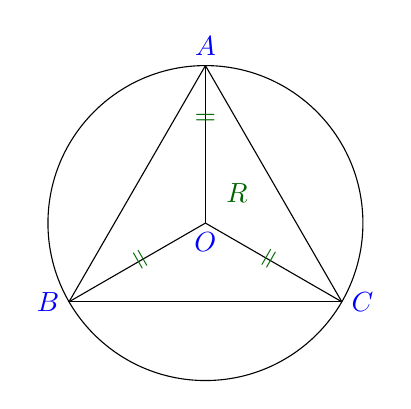
\begin{tikzpicture}
  \draw (0, 0) circle(2);
  \coordinate [label={[blue]above:$A$}] (A) at (0, 2);
  \coordinate [label={[blue]right:$C$}] (C) at (1.732, -1);
  \coordinate [label={[blue]left:$B$}] (B) at (-1.732, -1);
  \coordinate [label={[blue]below:$O$}] (O) at (0, 0);
  \draw (B) -- (C);
  \draw (A) -- (B);
  \draw (C) -- (A);
  \draw (O) -- (A);
  \draw (O) -- (B);
  \draw (O) -- (C);
  \coordinate [label={[label distance=0.2cm, black!60!green] above right:$R$}] (A2) at (0, 0);
  \node[label={[black!60!green]:$=$}] at ( $ (A)!0.5!(O) $ ) (A1) {};
  \node[label={[black!60!green, rotate=60, yshift=-.2cm, xshift=-0.1cm]:$=$}] at ( $ (C)!0.5!(O) $ ) (C1) {};
  \node[label={[black!60!green, rotate=120, yshift=-.2cm, xshift=-0.1cm]:$=$}] at ( $ (B)!0.5!(O) $ ) (B1) {};
\end{tikzpicture}
\end{document}
